\documentclass[a4paper,12pt]{article}
\usepackage[francais]{babel}
\usepackage[T1]{fontenc}
\usepackage[utf8]{inputenc}
\usepackage{pslatex}
\usepackage{url}
\usepackage{graphicx}
\usepackage{lscape}
\selectlanguage{francais}


\title{Rapport de Soutenance 2}
\author{
Ihy Group : \\
deguil\_x (Xavier Deguillard)\\
genite\_n (Nicolas Geniteau)\\
sezer\_s (Stephane Sezer)\\
wagnac\_t (Teddy Wagnac)
}

\begin{document}

\maketitle

\newpage

\section*{Introduction}

\newpage

\tableofcontents

\newpage

\section{Travail accompli}
	\subsection{Lecture du format}
Un pr\'erequis la cr\'eation d'un codec est sa lecture, le format doit
pouvoir \^etre lu tel quel, et non pas d\'ecompress\'evers un fichier wav pour
pouvoir ensuite le lire, on
perdrait alors tous int\'er\^et d'un tel format. Il faut donc mettre en place un
syst\`eme de ``streaming'' dans lequel la d\'ecompression et la lecture sont
simultan\'es.
		\subsubsection{Architecture du streaming}
La premi\`ere id\'ee qui vient à l'esprit, est d'attendre qu'une partie de la
musique soit lue pour commencer à d\'ecompresser puis lire ce que l'on vient de
d\'ecompresser. Malheureusement, cette implantation naïve ne fonctionne tout
simplement pas. En effet, d\'ecompresser un ``chunk'', c'est-à-dire un bout de la
musique, n'est pas une op\'eration instantan\'e, et donc par cons\'equent, la lecture
aurait marqu\'eun temps d'arr\^et à la fin de chaque chunk, correspondant à la
dur\'ee de d\'ecompression dudit chunk.\\
Pour pallier à ce probl\`eme il faut threader la d\'ecompression, à l'aide de deux
processus s\'epar\'es. Le premier processus va d\'ecompresser les chunks pendant que
le second va lire les chunks que le premier processus aura d\'ecompresser. Comme
la d\'ecompression dure moins longtemps que la lecture, il n'y a pas de temps
d'arr\^et notable lors d'un changement de chunk.\\
Pour mettre en place cette solution, il nous a fallu penser de façon parall\`ele,
en effet si la programmation s\'equentielle va de soit, il n'en est pas de m\^eme
pour la programmation parall\`ele. Et la se pose le premier probl\`eme, comment
communiquer entre ces deux processus?\\
		\subsubsection{Le buffer}
Ce qui ici est essentiel, est une structure de donn\'ees partag\'ees entre les
deux processus. Pour cela, un buffer est
tout appropri\'e. En effet, lorsque le processus de lecture a besoin de donn\'ees
d\'ecompress\'ees, il va simplement r\'ecup\'erer le prochain \'el\'ement du buffer, et
lorsque le processus de d\'ecompression a fini de d\'ecompresser, il va tout
simplement ajouter les donn\'ees dans le buffer. On voit ici clairement qu'un
buffer n'est qu'une simple structure de donn\'ee de type ``fifo''\footnote{first
in first out}, qui est souvent implant\'eavec une file.\\
Notre buffer est n\'eanmoins plus complexe qu'une simple file, en effet, il faut
qu'il puisse g\'erer les acc\`es concurrentiels de la part des deux processus. Pour
cela, on utilise des ``mutex'' pour prot\'eger les zones critiques, plus
pr\'ecis\'ement, l'ajout et le retrait d'un \'el\'ement. De plus, pour des raisons
d'\'economies de m\'emoire et d'activit\'edu processeur, il est judicieux que le
processus de d\'ecompression ne
soit pas toujours actif, en effet, lorsqu'un chunk est d\'ecompress\'e, il contient
uniquement des \'echantillons, tels qu'ils sont cod\'es dans un fichier wav, tout
d\'ecompresser en une seule fois reviendrai a avoir le fichier wav int\'egralement
en m\'emoire. En plus de cela, la lecture audio de notre format ne doit pas
impacter les performances de l'ordinateur. Pour r\'egler ces deux soucis, il
existe une solution plutôt simple, d\'efinir une taille maximum pour le buffer, et
lorsque celui-ci est plein, le processus de d\'ecompression va tout simplement
attendre que ce dernier se vide. La ``bonne taille'' a \'et\'ed\'etermin\'ee et est une
taille de buffer de trois, c'est-à-dire que le buffer ne peut contenir que
trois chunks.\\
		\subsubsection{Sortie audio}
Lorsque tout ceci fut mis en place, il ne restait plus qu'à utiliser ce que nous
avions commenc\'eà mettre en place à la soutenance derni\`ere, en pr\'evision de
cette lecture en streaming, la lecture d'un fichier wav. Ici, lorsque l'on
d\'ecompresse le ihy, on r\'ecup\`ere des bouts de wav, qui correspondent aux chunks
du format. Il ne reste alors plus qu'à les envoyer à libao, pour que ce dernier
nous le lise.
	\subsection{Le type half}
Un des gros probl\`emes que nous avions lors de la premi\`ere soutenance se situait
dans la place que prenait le stockage des \'echantillons sous forme de flotants.\\
Nous avons donc regl\'ele probl\`eme en utilisant le type half float qui n'existe
pas nativement en C.\\
Pour rappel, un flotant demi-precision est cod\'esur 16 bits, le premier servant
à definir le signe, les 5 suivants, l'exposant et les 10 derniers, la
mantisse.\\
Pour impl\'ementer ce type, nous avons utilis\'eles bit fields qui permettent de
d\'efinir une structure contenant (pour notre cas) des entiers non-sign\'es de n
bits, n'\'etant pas forc\'ement multiple de 8.\\
Les conversions float vers half et half vers float sont effectu\'ees en utilisant
une union : le sch\'ema d'un half est calqu\'esur un uint16\_t et est stock\'etel
quel dans le fichier de sortie.\\
Nous revenons donc à un fichier de taille identique au wav d'entr\'ee (en effet,
dans la tr\`es grande majorit\'edes cas, les \'echantillons sont cod\'es sur des
entiers de 16 bits dans un fichier wav).
	\subsection{Ondelettes}
A la soutenance prec\'edente, nous avions implement\'el'ondelette de
haar. Il s'agit de l'ondelette la plus simple à mettre en oeuvre mais
n'est pas la plus adapt\'ee pour la compression d'un signal audio.
Nous avons donc voulu en tester une autre. De nombreuses recherches
nous ont appris que la famille d'ondelettes de Daubechies donnait en
g\'en\'eral de bons r\'esultats mais que cela pouvait varier en fonction du
signal à compresser.\\
\subsubsection{Ondelettes de Daubechies}
Les ondelettes de Daubechies est une famille d'ondelettes respectants
certaines propriet\'ees bien pr\'ecises. Il s'agit de l'ondelette ayant le
plus petit support compact pour un nombre choisi de moments nuls. Pour
p moments nuls, le support de l'ondelette correspondante est de 2p. En
effet, il a \'et\'edemontr\'epar Ingrid Daubechies que toute ondellette à
p moments nuls a au moins 2p coefficients non nuls. Or les ondelettes
de Daubechies en ont exactement 2p. On peut donc dire qu'elles sont
optimales en ce qui concerne les moments nuls.\\
Il existe donc une infinit\'ed'ondelettes de cette famille qui sont
caracteris\'es par le nombre de moments nuls. Haar est par exemple une
ondelette de Daubechies avec un seul moment nul. Il ne reste donc plus
qu'à implementer cette ondelette pour un p quelconque.
\subsubsection{Impl\'ementation des ondellettes de Daubechies}
L'impl\'ementation de ces ondelettes nous ont caus\'ede nombreux
probl\`emes que nous n'avions pas pr\'evus.\\
Premi\`erement, la compr\'ehension math\'ematique de cet outil n'a pas \'et\'e
facile car il nous manquait encore des bases (tel que les S\'eries de
Fourriers que nous voyons que maintenant). Heuresement notre
professeur de mathematiques nous a conseill\'eun excelent livre sur les
ondelettes de Stephane Mallat qui nous a permis de combler certaines
de nos lacunes. Une fois que nous avions compris les differents
th\'eor\`emes, il fallait encore les transformer en algorithmes
utilisables
dans notre projet. Ca a \'et\'eplus dur que ce que nous pensions.\\
Là, nous avons rencontr\'eun nouveau probl\`eme auquel nous n'avions pas
pens\'e: les coefficients de bords. En effet, le concept des ondelettes
est un
principe math\'ematique qui s'applique sur un signal infini. Or dans
notre cas, le signal a bien \'evidement un d\'ebut et une
fin. Concr\'etement, pour la transform\'ee par ondelette, on a besoin des
valeurs prec\'edantes pour les premi\`eres valeurs et les suivantes pour
les derni\`eres valeurs alors qu'elles n'existent pas. Il existe trois
m\'ethodes pour pallier ces effets de bords. La premi\`ere consiste à
rendre le signal p\'eriodique et de le rendre cyclique. C'est assez
simple de le mettre en place mais cela entraine de grands coefficents
aux extremit\'es et n'ont plus r\'eellement de sens physique. Ce n'est
donc
pas adapt\'epour la compression du signal.\\
Une deuxi\`eme solution existe mais uniquement sur les ondelettes
sym\'etriques or il a \'et\'eprouv\'eque Haar est la seule a l'\^etre. Or Haar
n'a pas ce probl\`eme d'effets de bords car son support est de seulement
2.\\
Nous avons adopt\'eune autre m\'ethode qui consiste a utiliser des
ondelettes de bords adapt\'ees, ayant le m\^eme nombre de moments nuls
afin d'\'eviter de grands coefficients de bords. Cette m\'ethode est celle
qui donne les meilleurs r\'esultats mais est aussi la plus dure à mettre
en oeuvre. Nous avons eu beaucoup de mal à cause du manque
d'informations sur cette technique.\\
Nous avons rencontr\'eun dernier probl\`eme algorithmique. En effet, la
formule g\'en\'eral de la transform\'ee par ondelette a une complexit\'ebien
trop elev\'ee (on arrivait à plusieurs heures pour la compression de
quelques minutes de musique). Nous avons donc du optimiser
l'algorithme, comme nous l'avions fait pour Haar, en fonction de
p.\\\\
Ces nombreux soucis nous ont donc quelque peu ralenti dans notre
avanc\'ee et pour le moment seul la compression avec l'ondelette de
Daubechies fonctionne correctement. Il restera donc encore a faire la
decompression pour la prochaine soutenance.
\subsection{Traitements des coefficients}
Une fois la transform\'ee par ondelette effectu\'e, nous recup\'erons un
grand nombres de coefficients qu'il faut encore traiter pour avoir une
bonne compression avec huffman. Pour que ce soit efficace, il faut
avoir un maximum de valeurs identiques. Pour cela, nous appliquons
pour le moment trois filtres diff\'erents.
\subsubsection{Suppression des coefficients de petites echelles}
La premi\`ere \'etape est de supprimer les coefficients correspondants aux
petites \'echelles. En effet ceux-ci influent globalement sur les hautes
fr\'equences qui ne sont pas perçu par l'oreille humaine. On peut donc
d\'ejà supprimer la moitier des coefficients.
\subsubsection{Suppression des coefficients proches de zero}
La deuxi\`eme \'etape est de supprimer tout les coefficients relativement
proche de z\'ero. Là encore ces coefficients agissent que tr\`es peu sur
le signal final. Il a donc fallut trouver une valeur limite pour
laquel on pouvait considerer que ces coefficients en dessous de cette
valeur \'etaient n\'egligeables pour l'oreille.
\subsubsection{Egalisation}
La derni\`ere \'etape est l'\'egalisation des valeurs. En effet Huffman est
efficace si on a de nombreuses valeurs similaires. On parcourt donc le
tableau de coefficients en recherchant les valeurs qui sont
relativement proches puis on les remplace par la valeur
moyenne. Encore une fois, il a fallut trouver cette limite.
	\subsection{Parallelisme}
La compression du signal audio avec notre codec est hautement paralelisable, sa
ns aucune modification \`a l'algorithme de base. En effet, la compresssion s'effec
tue par chunks, c'est \`a dire que les blocs de donn\'ees sont pris sequentiellement
 et trait\'es dans cet ordre.\\
Il suffit donc de traiter plusieurs chunks \'a la fois au lieu de se limiter a un 
seul.\\
Nous avions, lors de la soutenance precedente, present\'e les probl\`emes li\`es a l'utilisation des pthreads pour effectuer des calculs en parallele. En effet, le garbage collector n'\'etant pas thread-safe, nous avions droit \`a plusieurs segfaults et autres joyeusetes du genre. De plus, les threads caml ne peuvent utiliser
plusieurs processeurs, contrairement \`a ce aue vous nous aviez dit \`a la soutenance
pr\'ec\'edente. Pour nous en convaicre, nous avons tent\'e d'execut\'e en parall\`ele
deux fonctions factorielles (sans conflits d'acc\`es), et de regarder l'occupation
processeur pour apercevoir que Caml n'utilisait en effet qu'un seul coeur.\\
Pour r\'esoudre ce probl\`eme, nous utilisons donc des forks.
``Les camls'' etant parfaitement isol\'es, nous evitons tout probleme de garbage collector et nous pouvons ainsi effecuter les calculs de facon parfaitement parral\`ele.
		\subsubsection{Les pipes}
Pour comuniquer entre les processus cr\'ee avec les forks, qui ont chacun une m\'emoire s\'epar\'ee, nous devions trouver un moyen de partager les donn\'ees entre les processus.\\
En g\'en\'eral, la solution se nomme pipe. Mais malheuresement pour nous, un pipe
est trop petit (!!), en effet un chunk ne rentrait pas int\'egrallement dedans, pour la petite histoire, un chunk fait en g\'en\'eral plus de 65000 octets.
	\subsection{Huffman suite et fin}
À la derni\`ere soutenance, nous pouvions utiliser huffman, pour compresser des
donn\'ees, n\'eanmoins, nous n'avions pas \'ecrit le code pour la d\'ecompression, et
donc nous ne pouvions pas savoir si cela marchait r\'eellement, nous savions juste
que cela devrait marcher th\'eoriquement. Nous avons donc \'ecrit le code pour
d\'ecompresser Huffman, et bien sûr, cela n'a pas fonctionn\'ed\`es le d\'ebut (ça
aurait \'et\'etrop beau). En fait, la technique utilis\'ee à la compression, pour
l'\'ecriture \'etait mauvaise, apr\`es r\'e\'ecriture de cette partie du code, tout
marchait.\\
La technique utilis\'ee pour d\'ecompresser des donn\'ees qui ont \'et\'epr\'ec\'edemment
compress\'ees via Huffman est simple, on r\'ecup\`ere le prochain bit des donn\'ees
compress\'ees, puis si il s'agit d'un 0, on recommence le proc\'ed\'esur le fils
gauche de l'arbre, si c'est un 1, à droite. Enfin le caract\`ere non compress\'eest
celui que l'on trouve lorsque l'on arrive en racine de l'arbre de Huffman, que
l'on avait, à la compression, sauv\'edans le fichier. Pour d\'ecompresser
totalement le fichier, on recommence ce petit
proc\'ed\'etant qu'il y a des caract\`eres dans celui-ci.\\
Contrairement à notre premi\`ere id\'ee, Huffman n'est pas appliqu\'esur tout le
fichier, il n'y a pas un arbre unique pour tout le fichier. En fait, chaque
chunk poss\`ede son propre arbre de Huffman, cela permet d'avoir un arbre de
Huffman qui est beaucoup plus pr\'ecis et donc, de gagner en compression, en
contrepartie, l'arbre de
Huffman doit \^etre \'ecrit pour chaque chunk. Il fallait donc trouver le bon
compromis, afin d'avoir une compression optimale. À cause des ondelettes, la
taille d'un chunk doit \^etre une puissance de deux, les tests pour l'optimalit\'e
de Huffman ont donc \'et\'eassez facile à r\'ealiser. Sans avoir fait de tests (et
m\^eme avant d'avoir commencer Huffman), nous avions fix\'ela taille d'un chunk
comme \'etant \'equivalente à 65536 \'echantillons, et coup de chance pour nous, il
s'agit de la taille optimale pour Huffman, un chunk deux fois plus gros, ou deux
fois plus petit, grossis la taille du fichier final de quelques
kilo-octets.\\

\newpage

	\subsection{Interface graphique}
À la premi\`ere soutenance, nous avions une interface graphique basique avec une 
barre de progression et les boutons standard d'un lecteur audio. Cette derni\`ere 
nous a permis de nous familiariser avec cet outil qui n'est rien d'autre que 
GTK+. Maitenant, pour cette soutenance, notre interface à quelque peu \'evolu\'ee grâce 
notamment à l'int\'egration de cairo dans notre projet...
	\subsubsection{La structure de l'interface}
Dans notre premiere \'ebauche d'interface, nous utilisions des box pour placer les
diff\'erents widgets dans la fen\^etre. Mais ce n'est pas la meilleure solution si 
on veut placer ses widgets à des endroits pr\'ecis. Donc nous avons tout simplement 
d\'ecid\'ed'utiliser une Table de 9 lignes et 9 colonnes. En effet, c'est un container 
de GTK+ qui utilise une grille invisible pour attacher les widgets. Donc il suffit 
d'int\'egrer les widgets dans la table et de les positionner grâce à des coordonn\'es.
Ce qui est plus avantageux qu'une Box qui elle positionne les widgets quasiment 
al\'eatoirement. Grâce à cette table, notre interface d\'etient une barre de progression 
et les boutons standard d'un lecteur audio comme à la premi\`ere soutenance, mais aussi 
une barre de menu et une zone de dessin (nous y reviendrons plus tard). Pour les boutons, 
nous avons tout de m\^eme utilis\'eune Box pour les contenirs  avec une dimension pr\'ecise et un 
espace entre eux nul. Comme pour la derni\`ere soutenance, la jauge se remplit quand
le bouton "Play" est activ\'e, avec le m\^eme principe que la derni\`ere fois. De plus, nous avons une 
barre de menu qui ne contient pour le moment que l'option "File". Dedans, on peut y trouver les boutons
"New" qui servira certainement à cr\'eer une nouvelle playlist, "Open" qui lui servira à 
r\'ecup\'erer un fichier de format Ihy dans son disque afin de pouvoir l'ouvrir et enfin 
le bouton "Quit" qui permet tout simplement de fermer l'application.
	\subsubsection{La zone de dessin}
Pour cette soutenance, nous devions int\'egrer dans notre interface une zone afin
d'entamer le spectrographe. Pour se faire, nous avons d\'ecid\'ed'utilis\'eser cairo.
Cairo est une biblioth\`eque logicielle graphique libre qui d\'efinit une API de
rendu vectoriel 2D ind\'ependante du mat\'eriel. De plus, cairo est parfaitement
utilisable avec GTK+. Nous avons donc aujourd'hui, une zone de dessin de
dimension 500x500, en fond noir, avec pour le moment dedans, deux \'etoiles en
mouvement. La premi\`ere \'etoile, r\'ealise un mouvement de translation et rotatif 
grâce aux fonctions cairo-translate() et cairo-rotate() toute deux issues de la
biblioth\`eque de cairo. Tandis que la seconde \'etoile, elle, r\'ealise un
mouvement de translation et rotatif mais aussi un mouvement d'\'echelle qui
provoque une impression de va et vien de l'\'etoile dans la zone de dessin. Ce
mouvemente est r\'ealis\'egrâce à la fonction cairo-scale.\\
Cependant, cette petite zone de dessin nous a pos\'eprobl\`eme pour l'int\'egration dans
notre interface. En effet, la fonction qui permet de cr\'e\'ela zone de dessin avec
les biblioth\`eques de cairo ne cr\'ee pas un widget directement. Ce qui est quelque
peut emb\'etant car la fonction qui permet d'int\'egr\'eer quelque chose dans une table
n'accepte que les widgets. Par cons\'equent , nous d\'ecidons de cr\'eer un GdkPixmap
qui contiendra la zone de dessin et qui sera d\'etenue dans un widget grâce à la
fonction gtk-pixmap-new().  
	\subsubsection{Pour la prochaine fois...}
Donc, pour la derni\`ere soutenance, nous esp\'erons terminer l'interface avec
l'int\'egration d'une playlist, de la fonction qui dessine dans la zone de
dessin en fonction de la musique, et en activant quelques widgets en plus. Pour
le moment, voici notre interface actuelle :
\begin{center}
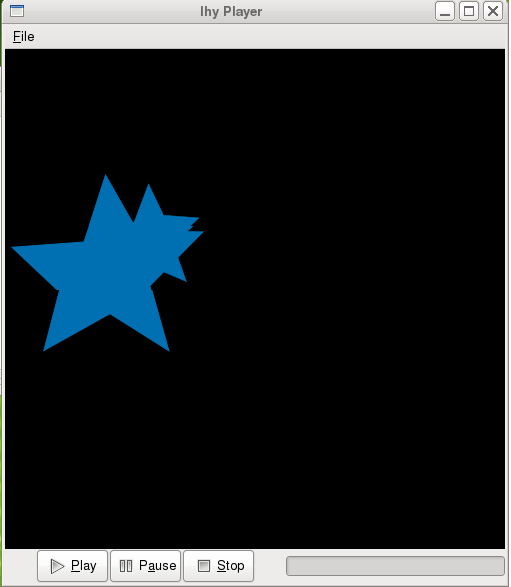
\includegraphics[scale=0.50]{img/Player.png}
\end{center}

\newpage

	\subsection{Portage sur iPhone}
Aujourd'hui, les codecs audio sont de plus en plus utilis\'es sur des
ordinateur poss\'edant une puissance plus que limite, j'ai nomm\'eles iPods
et d\'erives. Pour qu'un codec soit consid\`ere comme utilisable, il faut
qu'il puisse \^etre utilise sur ces plateformes, cela montre qu'il n'est
pas n\'ecessaire d'avoir un ordinateur tr\`es puissant pour pouvoir lire le
format. C'est \'egalement une preuve d'un codec bien r\'ealise, celui ci
\'etant alors portable et donc th\'eoriquement lisible sur tous les
appareils.\\
L'ann\'ee derni\`ere apple a sorti un SDK\footnote{software developpement
kit} permettant de d\'evelopper des applications pour l'iPhone\footnote{Lorsque
l'on parle d'iPhone, on parle \'egalement d'iPod Touch, qui sont identiques au
niveau plateforme de d\'eveloppement}, ceci en
utilisant les outils ainsi que la documentation officielle, et ce de façon gratuite.
C'est l'occasion r\^ev\'ee de montrer que notre codec est a la fois
portable et l\'eger.\\
		\subsubsection{Reunir les outils}
Premi\`ere \'etape donc, absolument indispensable a la r\'ealisation du
portage, la mise en place d'un environnement de cross-compilation,
c'est-à-dire, un compilateur, et les outils associ\'es,  pouvant g\'en\'erer du code
pour iPhone, qui
tourne sur un ordinateur classique. Le SDK de apple en fournit un, mais
celui-ci est compatible uniquement avec MAC OSX Leopard, ce que nous ne
poss\'edons pas. Heureusement, la communaut\'e``underground'' de l'iPhone
est assez importante, en cherchant bien, on a r\'eussi a trouver un
tutoriel expliquant comment se construire un
``toolchain''\footnote{logiciel et headers complet pour compiler un
programme} int\'egral sur Linux. Apr\`es cela, nous pouvions compiler et lancer un
simple Hello World sur l'iPhone.\\
Mais voila, notre projet n'est pas uniquement fait de C, mais \'egalement
de OCaml. Il a donc fallu trouver une façon de cr\'eer un compilateur
cross-compilateur OCaml
pour l'iPhone. On a \'egalement trouv\'eun tutoriel tr\`es d\'etaill\'e, fournissant les
patchs a appliquer aux sources de OCaml, pour que celui-ci g\'en\`ere du code pour
iPhone.
		\subsubsection{Compiler le projet}
Notre projet ne poss\'edant que tr\`es peu de d\'ependance externes, la
compilation s'est bien d\'eroul\'ee, sauf sur la seule d\'ependance : libao, la
biblioth\`eque nous permettant de lire du son. Apr\`es l'avoir retire du
projet, nous avons teste le bon fonctionnement des autres composants du
projet, c'est-à-dire la compression et la d\'ecompression. Cela a
fonctionn\'edu premier coup, chose a laquelle je ne m'attendais pas.\\
		\subsubsection{La sortie audio}
Libao ne compilant pas, il nous fallait imp\'erativement trouver une autre
solution pour lire du son. En fouillant dans la documentation de Apple, je suis
tomb\'esur un article montrant comment utiliser les ``Audio Queues'', qui est
d\'ecrit comme \'etant ``la solution pour lire vos sons de façon asynchrone''. La
description colle exactement avec l'utilisation qu'on veut en avoir.\\
Dans les grandes lignes, apple a implant\'ela notion d\'ecrite plus haut pour
les buffers audio, et l'a rendue utilisable via ces Audio Queues. La seule chose
à faire est de cr\'eer une fonction qui sera appel\'ee lorsque le lecteur audio aura
besoin de nouvelles donn\'ees. Dans notre cas, cette fonction va tout simplement
d\'ecompresser le fichier ihy et le renvoyer sous la forme d'un flux PCM.\\
Lorsque cela fut implanter, l'iPhone pouvait lire, de façon th\'eorique, notre
format. Restait à le v\'erifier sur l'iPhone. Et là oh surprise, cela
fonctionnait, de façon totalement fluide. 
	\subsection{Site web}
Ce dernier n'a pas beaucoup \'evolu\'e, au niveau de l'interface depuis la derni\`ere
soutenance. N\'eanmoins, des changements non visible ont \'et\'efait. En effet, à la
derni\`ere soutenance, le site n'\'etait absolument pas valide avec la norme w3c, et
pr\'esentait un total de 19 erreurs, cela faisait beaucoup pour une seule
page\ldots\\
De plus, des news ont \'et\'eajout\'ees, pour que les internautes puissent connaître,
sans à avoir à regarder le code et les messages d\'epos\'es sur le git, l'avancement
du projet, les nouvelles fonctionnalit\'es, ainsi que les futures. Une news fait
m\^eme office de tutoriel pour compiler et utiliser le codec ihy sur un iphone
(voir ci-dessus), cette derni\`ere expliquant tr\`es pr\'ecis\'ement les diff\'erentes
\'etapes à suivre pour que tout fonctionne.

\newpage

\section{Tâches pr\'evues}
	\subsection{Documentation}
Pour cette ultime soutenance, nous avons pr\'evu d'\'ecrire une documentation du
format, suffisamment d\'etaill\'ee pour que n'importe qui puisse lire et \'ecrire un
fichier ihy sans d\'ependre de notre code. Il s'agit d'un pr\'erequis pour
l'utilisation de n'importe quel codec. Seul les firmes multinationales
maîtrisant à la fois le syst\`eme d'exploitation et les logiciels, peut se
permettre de ne pas donner les sp\'ecifications d'un codec.\\
Cette documentation contiendra plusieurs choses. Premi\`erement, la description
compl\`ete des ``headers'' du format, ces derniers \'etant indispensable à la
d\'ecompression du fichier. Deuxi\`emement, une description des algorithmes
utilis\'es, ou pouvant \^etre utilis\'es. Et enfin, l'ordonnancement des donn\'ees dans
le fichier compress\'e, comme par exemple, la façon dont l'arbre de Huffman est
stock\'e.
	\subsection{Comparaison entre les codecs}
Un \'el\'ement indispensable lors de la finalisation d'un codec audio (ou vid\'eo),
est sa comparaison avec les codecs existants. En effet, un nouveau codec ne
faisant rien de nouveau, compressant moins bien, ou ayant une qualit\'eà l'\'ecoute
moins bonne a peu de chances d'\^etre utilis\'e.\\
Il faudra donc, montrer les points forts de notre codecs fasse aux concurents
que sont par exemple le mp3, ogg, wma, etc. Tout en essayant de masquer au
maximum les points faible de notre codec\footnote{Cette partie aurait pu \^etre
nomm\'ee ``Publicit\'e''}.\\
Les points compar\'es seront donc, la qualit\'ed'\'ecoute, un facteur extr\^emement
objectif, ne pouvant \^etre chiffr\'e, la taille du fichier final, le spectre audio,
qui devrai confirmer les r\'esultats du premier test, et enfin, la rapidit\'ede
compression et de d\'ecompression, ainsi que la charge CPU lors de la lecture d'un
fichier.

\newpage

\section*{Conclusion}

\end{document}
